\chapter{Calculus of Communicating Systems}
Dati due processi $p_1$ ed $p_2$ si ha che essi sono specificati in
\textbf{esecuzione concorrente} con l'utilizzo della seguente notazione:
\begin{equation}
    p_1 | p_2 \ \text{dove} \ p_1, p_2 \in Proc_{CCS}
\end{equation}
L'esecuzione in concorrenza può portare a diverse complicanze qualora non venga
rispettato, per esempio, un certo ordine di esecuzione. Si ha quindi il
\textbf{non determinismo}, ovvero il risultato ottenuto dall'esecuzione dei
programmi dipende dall'ordine di esecuzione di essi. Inoltre, si perde la
composizionalità dei processi.
\begin{esempio}[\textbf{Non determinismo e nessuna composizionalità}]
    Supponiamo di avere due programmi $p_1$ e $p_2$ definiti nel seguente
    modo:
    \begin{equation}
        \begin{aligned}
            p_1 =\{x = V\} x = 2 \{x = 2\} \\
            p_2 =\{x = V\} x = 3 \{x = 3\}
        \end{aligned}
    \end{equation}
    con $V$ che indica un qualunque valore.

    L'esecuzione in parallelo di questi due programmi mi permette di ottenere i
    seguenti risultati:
    \begin{equation}
        \{x = V\} \ p_1 | p_2 \ \{x = 2 \lor x = 3\}
    \end{equation}
    avendo quindi una situazione di non determinismo. Inoltre, definendo un nuovo
    programma $p_1'$ possiamo osservare come la proprietà di composizionalità non
    risulta più valida.
    \begin{equation}
        p_1' = \{x = V\} \ x = 1; x = x + 1 \ \{x = 2\}
    \end{equation}
    Se proviamo a sostituire questo programma al posto di $p_1$ otteniamo:
    \begin{equation}
        \{x = V\} \ p_1' | p_2 \ \{x = 2 \lor x = 3 \lor x = 4\}
    \end{equation}
\end{esempio}
Per mantenere il principio di composizionalità si cambia linguaggio di
rappresentazione. Per modellare sistemi concorrenti esistono diverse cose:
\begin{itemize}
    \item \textbf{Algebre di processi}: CCS e CSP
    \item \textbf{Automi a stati finiti}: tutti gli automi a stati finiti e i
          riconoscitori di linguaggi, ricadono anche i sistemi di transizione
          etichettati, quest'ultimi utili per modellare la semantica interleaving
          delle algebre dei processi.
    \item \textbf{Reti di petri}
\end{itemize}
\section{Algebre dei processi}
Hoare ha introdotto un nuovo paradigma di programmazione, il paradigma \textbf{CSP}
(\textit{Communicating Sequential Processes}). In questo paradigma non si ha
più una memoria condivisa, ma un insieme di processi ciascuno con una sua memoria
privata. Si ha un'interazione tra processi tramite lo scambio di messaggi del
tipo hand-shacking, avendo quindi la sincronizzazione basata sullo scambio
di informazioni. Viene fatto anche un processo particolare rappresentante la
memoria condivisa. Avremo quindi:
\begin{equation}
    x \ | \ p_1 \ | \ p_2
\end{equation}
dove $x$ che rappresenta la memoria condivisa dai due processi.

Un diverso paradigma è quello proposto da Milner, il quale propose il lambda
calcolo ($\lambda$-calcolo) per passare dal paradigma sequenziale a quello
concorrente. In questo si studia in modo approfondito la composizionalità,
sfruttando la composizione tra funzioni, cercando di non perderla nel concorrente.
Introduce quindi una sorta di $\lambda$-calcolo concorrente, introducendo il
\textbf{CCS} (\textit{Calculus of Communicating Systems}), in cui pensa ad un
calcolo algebrico per sistemi comunicanti. Adotta anche lui un paradigma che
studia un sistema formato da componenti, chiamati processi. Questi processi
comunicano tramite la sincronizzazione delle operazioni. Per la gestione di
queste si utilizza la seguente notazione:
\begin{itemize}
    \item \textbf{$a$}: indichiamo un processo generico che invia il messaggio.
    \item \textbf{$\overline{a}$}: indichiamo un processo generico che riceve.
\end{itemize}
Un \textbf{sistema}, quindi, è un insieme di processi il cui comportamento è
gestito da un calcolo algebrico, si punta alle algebre di processi, ovvero
linguaggi di specifica di sistemi concorrenti che si ispirano al calcolo dei
sistemi comunicanti.

I messaggi di scambio corrispondono ad uno scambio di valori di variabili e questo
è rappresentabile dall'algebra. Utilizzando questa tecnica, i processi possono
interagire anche con l'ambiente esterno attraverso delle porte. Sfruttando
questa tecnica non si ha più un sistema chiuso.

Dato un sistema $P$, si scrive:
\begin{equation}
    P = p_1 \ | \ p_2 \ | \ p_3
\end{equation}
se $P$ è formato dai processi $p_1$, $p_2$ e $p_3$, processi che sono interagenti
a due a due. Ogni processo ha comunque una memoria privata.

Milner risolve il problema della \textit{composizionalità} tramite l'uso di
diverse porte che permettono ad un processo di comunicare con altri o con
l'ambiente esterno. Quindi ogni processo può essere visto come un insieme di
sotto-processi interagenti che però interagiscono tramite sincronizzazione con i
processi esterni tramite una porta. Bisogna comunque mantenere il comportamento
complessivo. Per il processo esterno è come se sostituissi il processo con cui
comunica con il suo sotto-processo. Si introduce il concetto di
\textbf{equivalenza all'osservazione}, che permette di sostituire un processo
$p_i$ con uno $p_i'$ se sono equivalenti rispetto all'osservazione, ovvero se e
solo se un qualsiasi osservatore esterno non è in grado di distinguere i due
processi.

Con il termine \textit{osservare} ci si riferisce all'interazione con il sistema
dove agisce il processo. Questo deve essere valido per ogni possibile osservatore.
Se questo è garantito la sostituzione di un processo non va a modificare
l'esecuzione complessiva, senza incorrere in deadlock o altre problematiche.
Per verificare l'equivalenza esistono diverse tecniche tra cui la
\textbf{bisimulazione}.
\section{Labeled Transition System}
Per modellare la semantica interleaving delle algebre dei processi si utilizzano
i \textbf{Labeled Transition System} (LTS).
\begin{definizione}[\textbf{Labeled Transition System}]
    Possiamo definire un \textbf{Labeled Transition System} (\textit{LTS}) come
    un automa che specifica il comportamento di un processo. Esso è definito a
    partire da una quadrupla:
    \begin{equation}
        LTS = (S, Act, T, s_0)
    \end{equation}
    dove:
    \begin{itemize}
        \item \textbf{$S$}: rappresenta un insieme di stati, che a differenza
              degli automi può non essere finito.
        \item \textbf{$Act$}: è un insieme delle possibili azioni (possono essere
              nomi o simboli).
        \item \textbf{$T$}: è una relazione definita come
              $T \subseteq S \times Act \times S$ tale che:
              $$(s, a, s') \in T \equiv s \xrightarrow{a} s'$$
        \item \textbf{$s_0$}: rappresenta lo stato iniziale. Questo campo non
              sempre è presente.
    \end{itemize}
\end{definizione}
La transizione $s \xrightarrow{a} s'$ può essere estesa a:
\begin{equation}
    s \xrightarrow{w} s', \ \text{con} \ w \in Act^*
\end{equation}
\begin{dimostrazione}
    È possibile dimostrare questa estensione per induzione:
    \begin{itemize}
        \item \textbf{Base}: $w = \varepsilon$, ovvero $w$ è la stringa vuota,
              allora $s = s'$.
        \item \textbf{Passo induttivo}: $w = a \cdot x$ con $a \in Act$ e
              $x \in Act^*$, allora:
              \begin{equation}
                  s \xrightarrow{a\cdot x} s' \iff s \xrightarrow{a} s''
                  \xrightarrow{x} s'
              \end{equation}
    \end{itemize}
\end{dimostrazione}
Quindi si può definire l'estensione:
\begin{equation}
    \xrightarrow{}  = \bigcup_{a \in Act} \xrightarrow{a}
\end{equation}
e definire la chiusura transitiva e riflessiva:
\begin{equation}
    \xrightarrow{\ast}  = \bigcup_{w \in Act^{\ast}} \xrightarrow{w}
\end{equation}
\section{CCS - Calculus of Communicating Systems}
Il CCS è un linguaggio di specifica per sistemi concorrenti. È un linguaggio che
astrae tutte le questioni legate ai dati.
\begin{definizione}[\textbf{Calculus of Communicating Systems}]
    Per definire il \textbf{Calculus of Communicating Systems} (CCS) \textit{puro}
    dobbiamo definire:
    \begin{itemize}
        \item  $K$: insieme di nomi di processi, che possono anche essere
              simboli di un alfabeto.
        \item  $A$: insieme di nomi di azioni.
        \item $\overline{A}$: insieme di co-nomi di azioni contenute
              in $A$:
              \begin{equation}
                  \overline{A} = \{\overline{a} \ | \ a \ \in \ A\} \Rightarrow
                  \overline{\overline{a}} = a
              \end{equation}
        \item $Act = A \ \cup  \ \overline{A} \ \cup \ \{\tau\}$: insieme delle
              azioni, dove $\tau \notin A$ corrisponde all'\textbf{azione di
                  sincronizzazione} tra $a$ e $\overline{a}$, ovvero la
              sincronizzazione è avvenuta. $A$ e $\overline{A}$ sono azioni
              \textbf{osservabili} e si indica con: $$L = A \cup \overline{A}$$
              mentre $\tau$ non è osservabile. Ricordando che osservare un'azione
              significa poter interagire con essa.
    \end{itemize}
\end{definizione}
Alla fine un processo CCS è definito così:
\begin{equation}
    P = a.P, P \in K
\end{equation}
Significa che $P$ esegue $a$ e si comporta come $P$ (ricorsione).
\begin{equation}
    P_1 = a.P_2, P_1, P_2 \in K
\end{equation}
Ogni processo CCS può essere descritto da un LTS associato e attraverso delle
regole di inferenza strutturate nel seguente modo:
\begin{equation}
    \frac{Premesse}{Conseguenze}
\end{equation}
Dare un significato tramite LTS, regole di inferenza e sintassi, è detto
semantica operazionale strutturale.
\begin{itemize}
    \item \textbf{Processo vuoto}: è definito come $P = \textbf{Nil}$ o 0 che ha
          un solo stato senza transazioni.
          \begin{center}
              \begin{tikzpicture}[shorten >=1pt,node distance=2cm,on grid,auto]
                  \node[state] (q_0) {$Nil$};
              \end{tikzpicture}
          \end{center}
    \item \textbf{Prefisso}: in cui si ha $\alpha \cdot P$ dove $P \in Proc_{CCS}$
          e $\alpha \in Act$. Questo può essere rappresentato mediante inferenza
          nel seguente modo:
          \begin{equation}
              \frac{}{\alpha \cdot P \xrightarrow{\alpha} P}
          \end{equation}
          \begin{center}
              \begin{tikzpicture}[shorten >=1pt,node distance=2cm,on grid,auto]
                  \node[state] (q_0) {$\alpha\cdot p$};
                  \node[state] (q_1) [right=of q_0] {$p$};
                  \path[->]
                  (q_0) edge  node {$\alpha$} (q_1);
              \end{tikzpicture}
          \end{center}
    \item \textbf{Somma}: siano $p_1, p_2 \in Proc_{CCS}$ posso comporli
          utilizzando l'operatore $+$ nel seguente modo $p_1 + p_2$. In questo
          caso per definire le regole di inferenza necessito $\alpha, \beta \in
              Act$ e $p_1', p_2' \in Proc_{CCS}$:
          \begin{equation}
              \frac{p_1 + p_2 \xrightarrow{\alpha} p_1'}{p_1 + p_2
                  \xrightarrow{\alpha} p_1'}
              \ \ \lor \ \
              \frac{p_1 + p2 \xrightarrow{\beta} p_2'}{p_1 + p_2
                  \xrightarrow{\beta} p_2'}
          \end{equation}
          \begin{center}
              \begin{tikzpicture}[shorten >=1pt,node distance=2cm,on grid,auto]
                  \node[state] (q_0) {$p_1+p_2$};
                  \node[state] (q_1) [below right=of q_0] {$p_1'$};
                  \node[state] (q_2) [below left=of q_0] {$p_2'$};
                  \path[->]
                  (q_0) edge  node {$\alpha$} (q_1)
                  (q_0) edge  node [above left] {$\beta$} (q_2);
              \end{tikzpicture}
          \end{center}
          Questo caso può essere generalizzato per più processi. Posso avere
          $\sum_{i \in I} p_i$ avendo multiple somme di processi:
          \begin{equation}
              \frac{p_j \xrightarrow{\alpha} p_j'}{\sum_{i \in I} p_i
                  \xrightarrow{\alpha} p_j'}, \ j \in J
          \end{equation}
          \begin{center}
              \begin{tikzpicture}[shorten >=1pt,node distance=3cm,on grid,auto]
                  \node[state] (q_0) {$p_1+p_2+p_3$};
                  \node[state] (q_1) [below right=of q_0] {$p_1'$};
                  \node[state] (q_3) [below left=of q_0] {$p_3'$};
                  \node[state] (q_2) [below =of q_0] {$p_2'$};
                  \path[->]
                  (q_0) edge  node {$\alpha$} (q_1)
                  (q_0) edge  node[above left]{$\gamma$} (q_3)
                  (q_0) edge  node[above left] {$\beta$} (q_2);
              \end{tikzpicture}
          \end{center}
          Nel caso di $I = \emptyset$ avrò $\sum_{i \in I} p_i = Nil$. Nel momento
          in cui ho 2 processi in una somma che con la medesima azione hanno 2
          transizioni diverse allora si introduce un comportamento non
          deterministico perché non so quale dei due viene eseguito.

    \item \textbf{Composizione parallela}: indicata con il simbolo $p_1 | p_2$ e
          utilizzando le regole di inferenza:
          \begin{equation}
              \frac{p_1 \xrightarrow{\alpha} p_1'}{p_1 | p_2
                  \xrightarrow{\alpha} p_1' | p_2}
              \ \ \lor \ \
              \frac{p_2 \xrightarrow{\alpha} p_2'}{p_1 | p_2
                  \xrightarrow{\alpha} p_1 | p_2'}
              \ \ \lor \ \
              \frac{p_1 \xrightarrow{\alpha} p_1' \land p_2
                  \xrightarrow{\overline{\alpha}} p_2'}{p_1 | p_2
                  \xrightarrow{\tau} p_1' | p_2'}
          \end{equation}
          in quest'ultimo caso, non potremo più avere altre sincronizzazioni.
          \begin{center}
              \begin{tikzpicture}[shorten >=1pt,node distance=3cm,on grid,auto]
                  \node[state] (q_0) {\small{$a\cdot p_1'|\overline{a}\cdot p_2'$}};
                  \node[state] (q_1) [below right=of q_0] {\small{$a\cdot p_1'|p_2'$}};
                  \node[state] (q_3) [below left=of q_0] {\small{$p_1'|\overline{a}\cdot
                              p_2'$}};

                  \node[state] (q_2) [below right =of q_3] {\small{$p_1'|p_2'$}};
                  \path[->]
                  (q_0) edge  node {$\overline{\alpha}$} (q_1)
                  (q_1) edge  node {$\alpha$} (q_2)
                  (q_3) edge  node [below left]{$\overline{\alpha}$} (q_2)
                  (q_0) edge  node [above left]{$\alpha$} (q_3)
                  (q_0) edge  node [above left] {$\tau$} (q_2);
              \end{tikzpicture}
          \end{center}
    \item \textbf{Restrizione}: sia $L \subseteq A$. Si ha che:
          \begin{equation}
              p_{\setminus L}
          \end{equation}
          indica che il processo $p$ \textbf{non} può interagire con il suo
          ambiente con azioni in $L \cup \overline{L}$ ma le azioni in
          $L \cup \overline{L}$ sono locali a $p$:
          \begin{equation}
              \frac{p \xrightarrow{\alpha} p'}{ p_{\setminus L}
              \xrightarrow{\alpha} p'_{\setminus L}}
          \end{equation}
    \item \textbf{Rietichettatura}: ovvero il cambiamento di nome ad una componente,
          ad una certa azione, per poter riusare tale nome. Ho quindi una
          funzione $f$ tale che:
          \begin{equation}
              f: Act \to Act
          \end{equation}
          inoltre, deve sempre essere garantito che:
          \begin{itemize}
              \item $f(\tau) = \tau$
              \item $f(\overline{a}) = \overline{f(a)}$
          \end{itemize}
          Ho quindi $p_{[f]}$ tale che:
          \begin{equation}
              \frac{p \xrightarrow{\alpha} p'}{p_{[f]} \xrightarrow{f(a)} p_{[f]}'}
          \end{equation}
    \item $K = P$ con $K$ uguale al nome di processo e $P \in Proc_{CCS}$:
          \begin{equation}
              \frac{P \xrightarrow{\alpha} P' \land K = P}{K \xrightarrow{\alpha} P'}
          \end{equation}
\end{itemize}
Nel caso di composizione parallela posso eseguire le due operazioni o in una
sequenza o nell'altra. Ho quindi una simulazione sequenziale non deterministica
del comportamento del sistema dato dalla composizione parallela.

Per poter dire che una certa implementazione soddisfa ($\models$) una certa
specifica o se due implementazioni diverse soddisfano la stessa specifica ci
serve una relazione di equivalenza tra processi CCS, ovvero una relazione del
tipo:
\begin{equation}
    R \subseteq Proc_{ccs} \times Proc_{ccs}
\end{equation}
tale che sia \textit{riflessiva}, \textit{simmetrica} e \textit{transitiva}.

Bisognerà inoltre astrarre:
\begin{itemize}
    \item Gli stati e considerare le azioni $Act$.
    \item Dalle sincronizzazioni interne, ovvero dalle $\tau$.
    \item Rispetto al non determinismo.
\end{itemize}
Milner poi asserisce che $R$ deve essere inoltre una \textbf{congruenza} rispetto
agli operatori del CCS.
\begin{definizione}[\textbf{Congruenza}]
    Una relazione di equivalenza $R$ è una \textbf{congruenza} se e solo se:
    \begin{equation}
        \forall p, q \in Proc_{CCS} \land \forall c[\cdot] \ \text{contesto} \ CCS
    \end{equation}
    avendo quindi un \textbf{contesto}, un'espressione CCS con qualcosa di mancante,
    CCS sostituibile con qualcosa, allora:
    \begin{equation}
        \text{se} \ p\ R\ q \ \text{allora si ha} \ c[p] \ R \ c[q]
    \end{equation}
\end{definizione}
Con LTS perdo la concorrenza perché tutto viene eseguito come esecuzione
sequenziale non deterministica (semantica interleaving). Con le reti di Petri
si potrà simulare il fatto che sia parallelo.

Abbiamo visto come associare CCS a LTS passando per le regole di inferenza.
Ora consideriamo un sistema di processi che interagisce con l'ambiente allora
vogliamo sapere come trovare una relazione di equivalenza per sostituire un
processo con un altro.

Nel caso di un processo sequenziale basta sostituire il modulo con altro
rispettando i domini di I e O. Nel parallelo dobbiamo mantenere rispettate
le interazioni con l'ambiente. Quindi una relazione di equivalenza con una
congruenza rispetto agli operatori ccs.

Da una relazione di equivalenza $\simeq$ tra i processi $p, q \in Proc_{CCS}$ ci
si aspetta che:
\begin{itemize}
    \item $LTS(p)$ isomorfo $LTS(q)$ allora $p \simeq q$
    \item Si astraggono gli stati e si considerano solo le azioni.
    \item $p \simeq q \Rightarrow Tracce(p) = Tracce(q)$
    \item $p \simeq q$ allora $p$ e $q$ devono avere la stessa possibilità di
          generare deadlock nell'interazione con l'ambiente.
    \item $\simeq$ deve essere una congruenza rispetto agli operatori CCS, cioè
          deve essere possibile sostituire un sotto-processo con un suo equivalente.
\end{itemize}
\begin{definizione}[\textbf{Isomorfismo}]
    Dati due sistemi di transizione etichettati $LTS_1 = (Q_1, Act_1, T_1, q_{01})$
    e $LTS_1 = (Q_2, Act_2, T_2, q_{02})$, possiamo affermare che
    $LTS_1$ è \textbf{isomorfo} a $LTS_2$ se e solo se:
    \begin{itemize}
        \item $\alpha: Q_1 \to Q_2$ è una funzione biunivoca.
        \item $\beta: Act_1 \to Act_2$ è una funzione biunivoca.
        \item $\alpha(q_{01}) = q_{02}$
        \item $(q_1, a, q_2) \in Act_1 \iff (\alpha(q_1), \beta(a), \alpha(q_1'))
                  \in Act_2$
    \end{itemize}
\end{definizione}
Questa definizione è troppo stretta perché è come sostituire cose uguali.
Introduciamo quindi una relazione di equivalenza come $p \sim q \iff Tracce(p) =
    Tracce(q)$, per tracce si intende la stessa sequenza di azioni possibile.
\begin{definizione}[\textbf{Tracce}]
    Se $P \in Proc_{CCS}$ allora:
    \begin{equation}
        Tracce(P) = \{w \in Act^* \ | \ \exists P' \in Proc_{CCS}, \
        P \xrightarrow{w} P'\}
    \end{equation}
    dove:
    \begin{itemize}
        \item Se $w = \varepsilon$ allora $P =  P'$
        \item Se $w = x_1 \cdot x_2 \cdot \dots \cdot x_n$ con $x_i \in Act$
              $\exists P_1', P_2', \dots, P_n' \in Proc_{CCS}$ tale che:
              \begin{equation}
                  P \xrightarrow{x_1} P_1' \xrightarrow{x_2} \dots
                  \xrightarrow{x_n} P_n' = P'
              \end{equation}
    \end{itemize}
\end{definizione}
\begin{definizione}[\textbf{Equivalenza rispetto alle tracce}]
    Quindi $P_1 \stackrel{T}{\sim} P_2 \iff Tracce(P_1) = Tracce(P_2)$ come
    equivalenza rispetto alle tracce.
\end{definizione}
\begin{osservazione}
    Con l'equivalenza rispetto alle tracce si introducono le seguenti osservazioni:
    \begin{itemize}
        \item $LTS(p)$ isomorfo $LTS(q)$ implica $p \stackrel{T}{\sim} q$
        \item Si ha un'astrazione di stati.
        \item $p \stackrel{T}{\sim} q \iff Tracce(p) = Tracce(q)$
        \item È una \textbf{congruenza} tra gli operatori CCS.
        \item Non garantisce di preservare la stessa probabilità di deadlock (o
              assenza) nell'interazione con l'ambiente.
    \end{itemize}
\end{osservazione}
Lo studio delle tracce non è più sufficiente nel caso di sistemi concorrenti.
Si necessità quindi di una nozione più restrittiva.
\subsection{Bisimulazione forte}
Dal momento che l'equivalenza secondo la Traccia può portare a Deadlock
allora si utilizzerà l'uguaglianza secondo l'osservatore, ovvero se l'osservatore,
interagendo, non nota differenze. In una variante si chiama Bisimulazione,
perché devo poter distinguere tra le 2. In sostanza $M_1$ simula $M_2$ e $M_2$
simula $M_1$.
\begin{definizione}[\textbf{Relazione di Bisimulazione Forte}]
    Data una relazione binaria $R \subseteq Proc_{CCS} \times Proc_{CCS}$ è una
    relazione di \textbf{bisimulazione} (\textbf{forte}) ($\stackrel{Bis}{\sim}$)
    se e solo se $\forall p, q \in Proc_{CCS}: \ p R q$ vale che:
    \begin{itemize}
        \item $\forall \alpha \in Act = A \cup \overline{A} \cup \{\tau\}$ se ho
              $p \xrightarrow{\alpha} p'$ allora deve esistere un processo
              \begin{equation}
                  \exists q' \ \text{tale che} \ q \xrightarrow{\alpha} q' \
                  \text{e si ha} \ p'Rq'
              \end{equation}
        \item E viceversa, ovvero $\forall \alpha \in Act = A \cup \overline{A}
                  \cup \{\tau\}$
              se ho $q \xrightarrow{\alpha} q'$ allora deve esistere un processo
              \begin{equation}
                  \exists p' \ \text{tale che} \ p \xrightarrow{\alpha} p' \
                  \text{e si ha} \ p'Rq'
              \end{equation}
    \end{itemize}
    Due processi $p$ e $q$ sono fortemente bisimili, indicato con la notazione
    $p \stackrel{Bis}{\sim} q$ se e solo se $\exists R \subseteq Proc_{CCS} \times
        Proc_{CCS}$, relazione di bisimulazione forte tale che:
    \begin{equation}
        p R q \ \ \land \ \
        \stackrel{Bis}{\sim} = \bigcup \{R \subseteq Proc_{CCS} \times Proc_{CCS}
        \ | \ R \ \text{è una relazione di bisimulazione forte}\}
    \end{equation}
\end{definizione}
\begin{teorema}
    Se prendo $\stackrel{Bis}{\sim}  \subseteq Proc_{CCS} \times Proc_{CCS}$ si
    dimostra che è una relazione di equivalenza, ovvero è riflessiva, simmetrica
    e transitiva. Quindi:
    \begin{equation}
        p \stackrel{Bis}{\sim} q \Longleftrightarrow \forall \alpha \in Act \
        \text{se} \ p \xrightarrow{\alpha} p'
        \ \text{allora} \
        \exists q' \ \text{tale che} \ q \xrightarrow{\alpha} q' \ \land \ p'
        \stackrel{Bis}{\sim} q'
    \end{equation}
    e se:
    \begin{equation}
        q \xrightarrow{\alpha} q' \ \text{allora} \
        \exists p' \ \text{tale che} \ p \xrightarrow{\alpha} p' \ \land \ p'
        \stackrel{Bis}{\sim} q'
    \end{equation}
\end{teorema}
\begin{teorema}
    Se due processi sono fortemente bisimili allora sono sicuramente equivalenti
    rispetto alle tracce. Non vale il viceversa.
    \begin{equation}
        p \stackrel{Bis}{\sim} q \Rightarrow p \stackrel{T}{\sim} q
    \end{equation}
\end{teorema}
\begin{osservazione}
    Per vedere che due processi sono bisimili devo quindi, per ogni esecuzione,
    ottenere due processi ancora bisimili (potendo quindi fare le azioni
    corrispondenti da entrambe le parti).
\end{osservazione}
\begin{esempio}
    Consideriamo i processi $p_1 = a \cdot b \cdot Nil + a \cdot c \cdot Nil$ e
    $p_2 = a \cdot (b \cdot Nil + c \cdot Nil)$
    \begin{figure}[!ht]
        \centering
        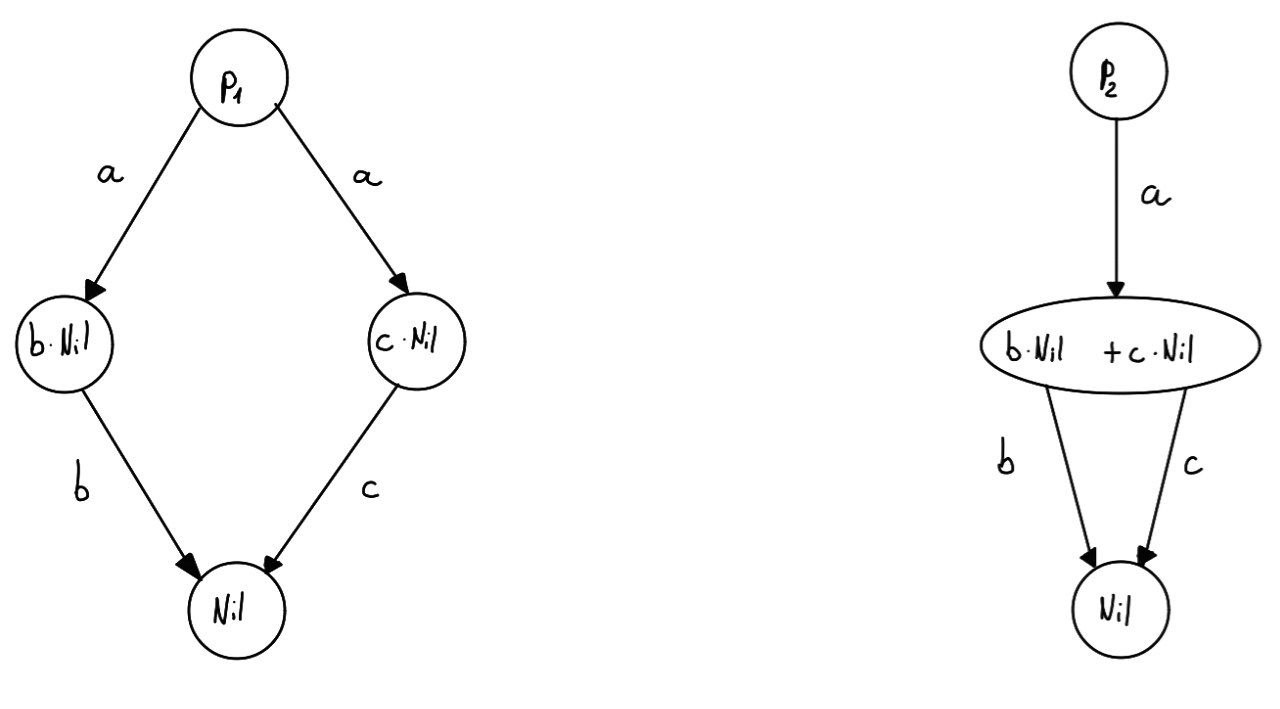
\includegraphics[scale=0.25]{img/ccs/Esempio1.png}
        \caption{LTS dei processi $p_1$ e $p_2$}
    \end{figure}
    Osserviamo subito che i due processi sono equivalenti rispetto alle tracce,
    difatti:
    \begin{itemize}
        \item $Tracce(p_1) = \{\varepsilon, a, a \cdot b, a \cdot c\}$
        \item $Tracce(p_2) = \{\varepsilon, a, a \cdot b, a \cdot c\}$
    \end{itemize}
    Vediamo se i due processi sono anche bisimili.
    \begin{itemize}
        \item Da $p_1$ possiamo eseguire l'azione $a$ e possiamo fare lo stesso
              anche da $p_2$. Dobbiamo però chiederci se gli stati di arrivo sono
              anche essi in relazione di bisimulazione.
        \item Gli stati interessati sono $b \cdot Nil$ e $b \cdot Nil + c \cdot
                  Nil$: dal primo possiamo eseguire $b$, che è fattibile anche
              dal secondo, ma dal secondo possiamo eseguire $c$, che non è
              eseguibile dal primo (la bisimulazione richiede che entrambi gli
              stati siano simili tra loro), dunque i due processi non sono bisimili.
    \end{itemize}
    Formalmente:
    \begin{itemize}
        \item $p_1 \xrightarrow{a} b \cdot Nil$
        \item $p_2 \xrightarrow{a} b \cdot Nil + c \cdot Nil$
    \end{itemize}
    $b \cdot Nil \stackrel{Bis}{\not\sim} b \cdot Nil + c \cdot Nil$ inoltre,
    possiamo osservare che: $b \cdot Nil \stackrel{T}{\not\sim} b \cdot Nil + c 
    \cdot Nil$
\end{esempio}
\begin{esempio}
    Consideriamo due processi che simulano dei buffer che possono contenere due
    elementi:
    \begin{itemize}
        \item $B_0^1 | B_0^1$ dove $B_0^1 = in \cdot B_1^1$ e $B_1^1 =
                  \overline{out} \cdot B_0^1$
        \item $B_0^2 = in \cdot B_1^2$, $B_1^2= \overline{out} \cdot B_0^2 + in
                  \cdot B_2^2$ e $B_2^2 = \overline{out} \cdot B_1^2$
    \end{itemize}
    \begin{figure}[!ht]
        \centering
        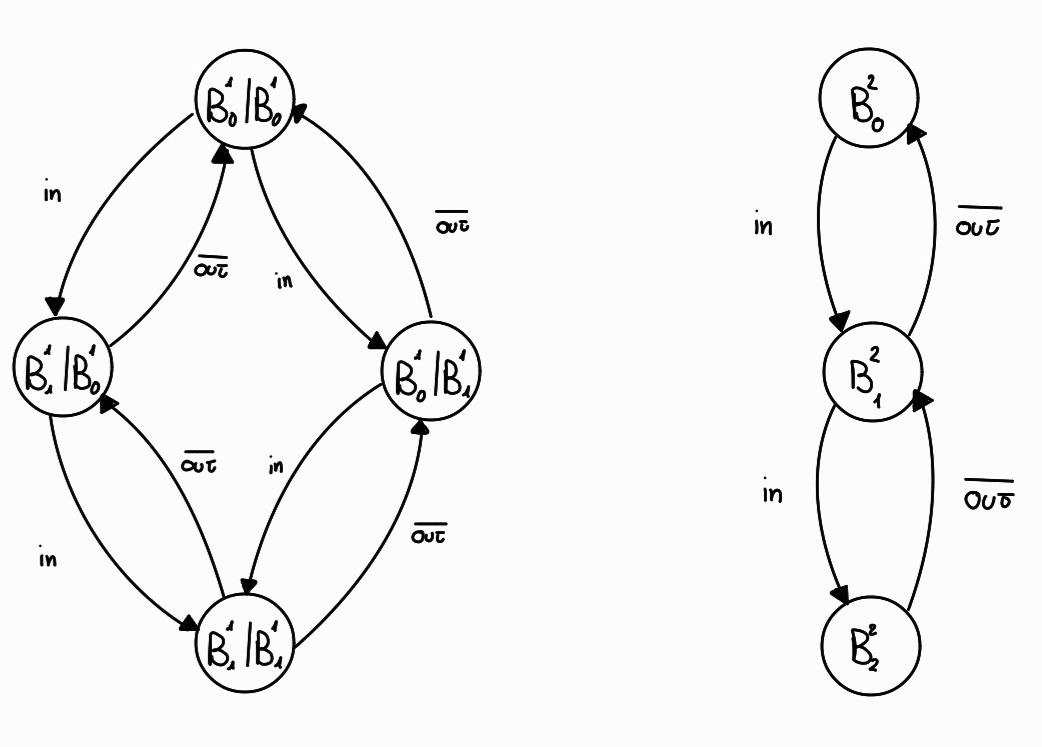
\includegraphics[scale=0.25]{img/ccs/Esempio 2.png}
        \caption{LTS dei processi $B_0^1 | B_0^1$ e $B_0^2$}
    \end{figure}
    In questo esempio, possiamo osservare che: $$(B_0^1 | B_0^1) \stackrel{Bis}{\sim} B_0^2$$
    $B_0^2$ può essere messo in relazione con $B_0^1| B_0^1$ in quanto se vado
    in uno tra $B_1^1 | B_0^1$ e $B_0^1 | B_1^1$ posso sempre fare $in$ e $\overline{out}$.
    Inoltre, Posso fare un discorso analogo per $B_2^2$ e $B_1^1 | B_1^1$.
    Essendo questi ultimi quindi bisimili lo sono anche il nodo centrale coi
    due possibili nodi nel caso della composizione e di conseguenza lo sono
    anche $B_0^2$ e $B_0^1 | B_0^1$.
\end{esempio}
La bisimulazione si può testare mettendo i due processi in parallelo e restringendo
le operazioni, se entrambi arrivano alla fine utilizzando la sincronizzazione
allora sono bisimili.
\begin{osservazione}
    La Bisimulazione forte è una congruenza anche rispetto agli operatori CCS,
    ovvero se $p, q \in Proc_{CCS} \land p \stackrel{Bis}{\sim} q$ allora:
    \begin{itemize}
        \item $\alpha.p \stackrel{Bis}{\sim} \alpha.q$
        \item $p + r \stackrel{Bis}{\sim}q + r$ e $r + p \stackrel{Bis}{\sim} r
                  + q, \forall r \in Proc_{CCS}$
        \item $p | r \stackrel{Bis}{\sim} q | r$ e $r | p \stackrel{Bis}{\sim} r
                  \forall r \in Proc_{CCS}$
        \item $\forall f: Act \to Act$ funzione di rietichettatura, se $p[f]
                  \stackrel{Bis}{\sim} q[f]$ allora $p \stackrel{Bis}{\sim} q$
        \item $p_{\setminus L} \stackrel{Bis}{\sim} q_{\setminus L}$ e $L \subseteq
                  Act$
    \end{itemize}
\end{osservazione}
\begin{osservazione}
    Inoltre valgono le seguenti proprietà:
    \begin{itemize}
        \item \textbf{Commutatività rispetto alla somma}: $p + q \stackrel{Bis}{\sim}
                  q + p$
        \item \textbf{Commutatività rispetto alla parallelizzazione}: $p | q
                  \stackrel{Bis}{\sim} q | p$
        \item \textbf{Associatività rispetto alla somma}: $(p + q) + r
                  \stackrel{Bis}{\sim} p + (q + r)$
        \item \textbf{Associatività rispetto alla parallelizzazione}: $(p | q) | r
                  \stackrel{Bis}{\sim} p | (q | r)$
        \item \textbf{Annullamento rispetto alla somma}: $p + Nil \stackrel{Bis}{\sim}
                  p$
        \item \textbf{Annullamento rispetto alla parallelizzazione}: $p | Nil
                  \stackrel{Bis}{\sim} p$
    \end{itemize}
\end{osservazione}
\begin{osservazione}
    Per ogni coppia $p, q \in Proc_{CCS}$ vale:
    \begin{itemize}
        \item $LTS(p)$ isomorfo $LTS(q)$ implica $p \stackrel{Bis}{\sim} q$
        \item Si ha un'astrazione di stati.
        \item $p \stackrel{Bis}{\sim} q \Rightarrow p \stackrel{T}{\sim} q \Rightarrow
                  \stackrel{Bis}{\sim} \subseteq \stackrel{T}{\sim}$
        \item È una congruenza tra gli operatori CCS.
        \item Preserva la stessa probabilità di deadlock (o assenza) nell'interazione
              con l'ambiente.
        \item $\stackrel{Bis}{\sim}$ è troppo restrittiva perché $a.b.Nil
                  \stackrel{Bis}{\not\simeq} a.\tau.b.Nil$. In sostanza $\stackrel{Bis}{\sim}$ e
              $\stackrel{T}{\sim}$ non astraggono le $\tau$.
    \end{itemize}
\end{osservazione}
\subsection{Bisimulazione debole}
La bisimulazione forte rischia di essere troppo restrittiva. Si passa quindi alla
definizione di \textbf{equivalenza debole rispetto alle tracce} $\stackrel{T}{\approx}$
e \textbf{bisimulazione debole} $\stackrel{Bis}{\approx}$.
La definizione di queste nuove relazioni obbliga a modificare la definizione
della funzione di transizione. La relazione di transizione debole è definita come:
\begin{equation}
    \Rightarrow \subseteq Proc_{CCS} \times Act \times Proc_{CCS}
\end{equation}
Possiamo rappresentare tale funzione come $p \stackrel{\alpha}{\Rightarrow} p'$ dove
$\alpha \in Act$ se e solo se:
\begin{itemize}
    \item Se $\alpha = \tau$ allora posso eseguire una sequenza qualsiasi, anche
          nulla, di $\tau$:
          \begin{equation}
              p \xrightarrow{\tau}^{\ast} p'\begin{cases}
                  p = p'
                                        & \text{se non ci sono } \tau \text{ da eseguire} \\
                  p \xrightarrow{\tau} p_1 \xrightarrow{\tau} \dots
                  \xrightarrow{\tau} p' & \text{altrimenti}
              \end{cases}
          \end{equation}
    \item Se $\alpha \in A \cup \overline{A}$ allora vale:
          $p \xrightarrow{\tau}^{\ast} \xrightarrow{\alpha} \xrightarrow{\tau}^{\ast}$
\end{itemize}
Come fatto per la relazione forte, definiamo la relazione di transizione per
sequenze di azioni $w \in Act^{\ast}$ come $p \stackrel{w}{\Rightarrow} p'$ se e solo se:
\begin{itemize}
    \item Se $w = \varepsilon$ oppure $w = \tau^{\ast}$ allora ho:
          \begin{equation}
              p \xrightarrow{\tau}^{\ast} p'
          \end{equation}
    \item Se $w = a_1\dots a_n$ con $a_i \in A \cup \overline{A}$ allora:
          \begin{equation}
              p \stackrel{a_1}{\Rightarrow} p_1 \stackrel{a_2}{\Rightarrow} \dots
              \stackrel{a_n}{\Rightarrow} p'
          \end{equation}
          dove ogni $a_i$ può essere preceduto/seguito da una qualsiasi sequenza
          di $\tau$.
\end{itemize}
\begin{definizione}[\textbf{Equivalenza debole rispetto alle tracce}]
    Definiamo l'\textbf{equivalenza debole rispetto alle tracce}, la quale è
    rappresentata come $p \stackrel{T}{\approx} q$ se e solo se:
    \begin{equation}
        tracce_{\Rightarrow} (p) = tracce_{\Rightarrow}(q) \ \text{ovvero} \
        \forall w \in (A \cup \overline{A}) \ \text{ho che} \ p
        \stackrel{w}{\Rightarrow} \iff q \stackrel{w}{\Rightarrow}
    \end{equation}
    quindi se i due processi possono eseguire la stessa sequenza di azioni.
\end{definizione}
Posso definire le tracce come:
\begin{equation}
    tracce_{\Rightarrow}(p) = \{w \in (A \cup \overline{A})^{\ast} | p
    \stackrel{w}{\Rightarrow}\}
\end{equation}
\begin{osservazione}
    In primis si ha che:
    \begin{equation}
        p \stackrel{T}{\sim} q \Rightarrow p \stackrel{T}{\approx} q \Rightarrow
        \stackrel{T}{\sim} \subseteq \stackrel{T}{\approx}
    \end{equation}
    Per ogni coppia $p, q \in Proc_{CCS}$ vale:
    \begin{itemize}
        \item $LTS(p)$ isomorfo $LTS(q)$ implica $p \stackrel{T}{\approx} q$
        \item Si ha un'astrazione di stati.
        \item È una congruenza tra gli operatori CCS.
        \item Non preserva la stessa probabilità di deadlock (o assenza)
              nell'interazione con l'ambiente.
    \end{itemize}
\end{osservazione}
\begin{definizione}[\textbf{Bisimulazione debole}]
    Data una relazione $R$ definita come $R \subseteq Proc_{CCS} \times Proc_{CCS}$.
    Dico che $R$ è una relazione di \textbf{bisimulazione debole} se e solo se:
    \begin{equation}
        \forall p, q \in Proc_{CCS} \ \text{tale che } p R q \ \text{vale che }
        \forall a \in Act
    \end{equation}
    \begin{itemize}
        \item Se $p \xrightarrow{a} p'$ allora $\exists q'$ tale che
              $q \stackrel{a}{\Rightarrow} q'$ e $p'Rq'$
        \item E deve valere anche il viceversa: $q \xrightarrow{a} q'$ allora
              $\exists p'$ tale che $p \stackrel{a}{\Rightarrow} p'$ e $p'Rq'$
    \end{itemize}
\end{definizione}
Due processi $p$ e $q$ sono in relazione di bisimulazione debole $p
    \stackrel{Bis}{\approx} q$
se e solo se esiste una relazione di bisimulazione $R$ tale che $p R q$ si ha che vale:
\begin{equation}
    \stackrel{Bis}{\approx} = \bigcup \{R | R \ \text{è di bisimulazione debole}\}
\end{equation}
\begin{esempio}
    Consideriamo i processi $r = a \cdot (b \cdot Nil + \tau \cdot c \cdot Nil)$
    e $k = a \cdot (b \cdot Nil + \tau \cdot c \cdot Nil) + a \cdot c \cdot Nil$.
    \begin{figure}[!ht]
        \centering
        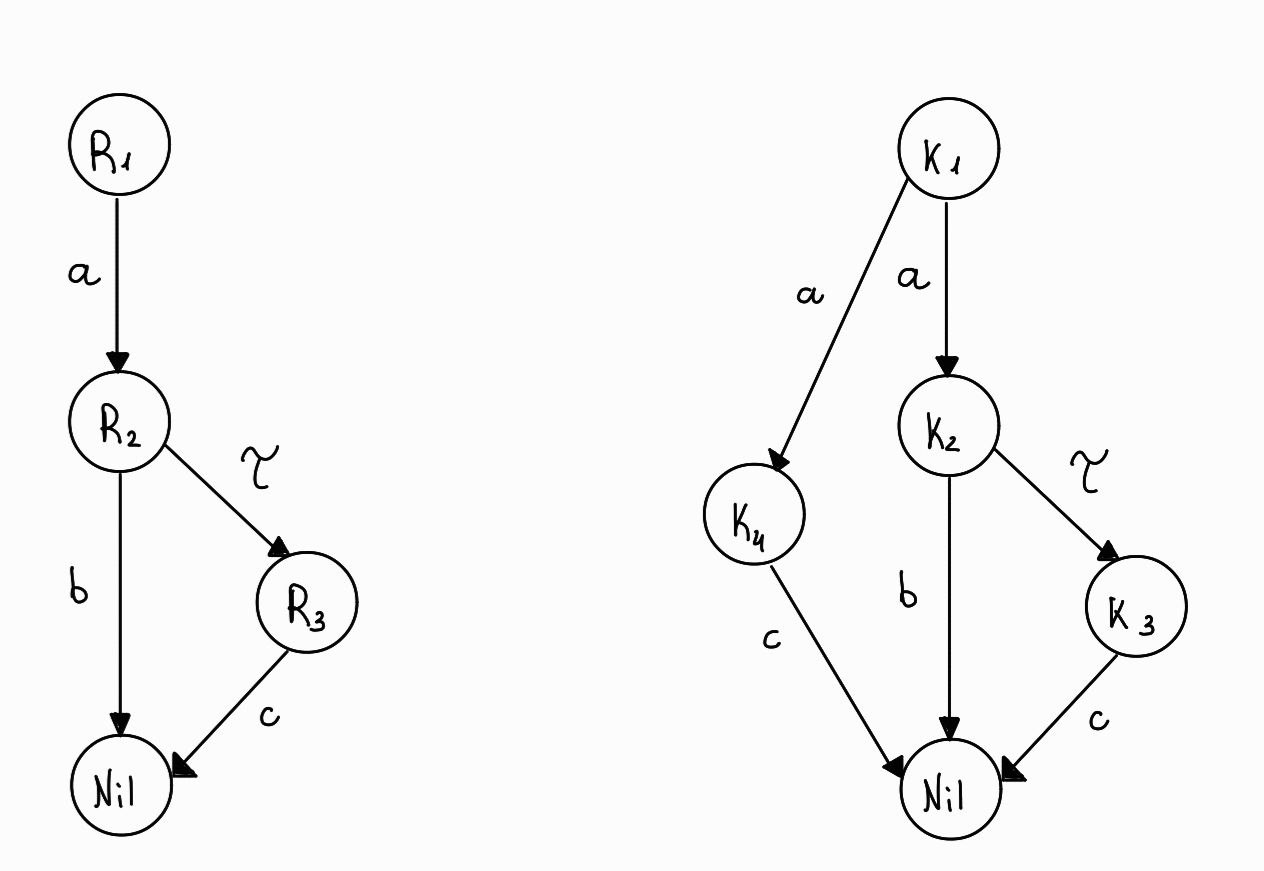
\includegraphics[scale=0.25]{img/ccs/Esempio3.png}
        \caption{LTS di $r$ e $k$}
    \end{figure}
    $$r \stackrel{Bis}{\approx} k$$
\end{esempio}
\begin{definizione}[\textbf{Processo deterministico}]
    Sia $p \in Proc_{CCS}$ è un processo deterministico se e solo se vale che:
    \begin{equation}
        \forall \alpha \in Act, \ p \xrightarrow{\alpha} p' \land p
        \xrightarrow{\alpha} p'' \Rightarrow p' = p''
    \end{equation}
\end{definizione}
\begin{osservazione}
    Siano $p, q \in Proc_{CCS}$, se $p, q$ sono deterministici e $p \stackrel{T}{\sim}
        q$ ($p \stackrel{T}{\approx} q$) allora $p \stackrel{Bis}{\sim}
        q$ ($p \stackrel{Bis}{\approx} q$).
\end{osservazione}
\begin{osservazione}
    Le proprietà della relazione di bisimulazione debole sono:
    \begin{itemize}
        \item È un'equivalenza.
        \item Preserva la possibilità di generare (o non generare) deadlock
              nell'interazione con l'ambiente (non ci sono problemi con i deadlock).
        \item Astraiamo dagli stati, azioni inosservabili ($\tau$) e dai cicli.
              \begin{equation}
                  Nil \stackrel{Bis}{\approx} \tau \cdot p
              \end{equation}
    \end{itemize}
\end{osservazione}
La bisimulazione debole \textbf{non} è una congruenza rispetto agli operatori CCS.
\begin{teorema}
    Se $p, q \in Proc_{CCS}$, $p \stackrel{Bis}{\approx} q$ allora:
    \begin{itemize}
        \item $\alpha . p \stackrel{Bis}{\approx} \alpha . q, \forall \alpha \in A$
        \item $p | r \stackrel{Bis}{\approx} q | r \land r | p \stackrel{Bis}{\approx}
                  r | q, \forall r \in Proc_{CCS}$
        \item $p[f] \stackrel{Bis}{\approx} q[f], \forall f: Act \to Act$ funzione
              di rietichettatura.
        \item $p_{\setminus L} \stackrel{Bis}{\approx} q_{\setminus L}, \forall
                  L \subseteq Act$
        \item Rispetto all'operatore $+$ e alla ricorsione questa cosa non è vera:
              \begin{equation}
                  \tau . a . Nil \stackrel{Bis}{\approx} a.Nil, \tau . a . Nil + b.Nil
                  \stackrel{Bis}{\not\approx} a.Nil + b.Nil
              \end{equation}
    \end{itemize}
\end{teorema}
\subsubsection{Congruenza}
Possiamo cercare la più grande relazione di congruenza $\stackrel{C}{\approx}$
che più si avvicina a $\stackrel{Bis}{\approx}$.
\begin{equation}
    \stackrel{C}{\approx} \subseteq \stackrel{Bis}{\approx} \subseteq Proc_{CCS}
    \times Proc_{CCS}
\end{equation}
Non sarà altro che una bisimulazione ristretta senza ricorsione e con processi
(agenti) finiti. Per fare ciò dovremo definire un insieme finito di assiomi $Ax$
che permetta di dimostrare la congruenza, tale che:
\begin{itemize}
    \item Ax \textit{corretto} ($Ax \vdash p = q \Rightarrow p \stackrel{C}{\approx} q$)
    \item Ax \textit{completo} ($p \stackrel{C}{\approx} q \Rightarrow Ax \vdash p = q$)
\end{itemize}
\begin{enumerate}
    \item \textbf{Legge associativa}:
          \begin{equation}
              p + (q + r) \stackrel{C}{\approx} (p + q) + r \ \text{e} \ p | (q | r)
              \stackrel{C}{\approx} (p | q) | r
          \end{equation}
    \item \textbf{Legge commutativa}:
          \begin{equation}
              p + q \stackrel{C}{\approx} q + p \ \text{e} \ p | q
              \stackrel{C}{\approx} q | p
          \end{equation}
    \item \textbf{Legge di assorbimento}:
          \begin{equation}
              p + p \stackrel{C}{\approx} p \ (\text{ma} \ p | p
              \stackrel{C}{\not\approx} p)
          \end{equation}
    \item $p + Nil \stackrel{C}{\approx} p$ e $p | Nil \stackrel{C}{\approx} p$
    \item $p + \tau \cdot p \stackrel{C}{\approx} \tau \cdot p$
    \item $\mu \cdot \tau p \stackrel{C}{\approx} \mu \cdot p$
    \item $\mu \cdot (p + \tau \cdot q) \stackrel{C}{\approx} \mu \cdot (p +
              \tau \cdot q) + \mu \cdot q$
    \item Se $p$ e $q$ sono delle somme: $p = \sum_{i} \alpha_i \cdot p_i$ e
          $q = \sum_{j} \beta_j \cdot q_j$,  $\alpha, \beta \in Act$:
          $$p | q \stackrel{C}{\approx} \sum_{i} \alpha_i (p_{i} | q) + \sum_{j}
              \beta_{j} \cdot (p|q_{j}) + \sum_{\alpha_i = \overline{\beta}_{j}}
              \tau \cdot (p_{i} | q_{j})$$
          (\textbf{Teorema di espansione di R. Milner}) Questo assioma mi permette
          di rappresentare la composizione parallela come la somma di tutte le
          possibili alternative che si hanno con l'operazione di composizione
          parallela.
    \item $p[f] \stackrel{C}{\approx} \sum_{i} f(\alpha_i) \cdot (p_{i} [f])$ $\forall f$
          funzione di etichettatura.
    \item $p_{\backslash L} \stackrel{C}{\approx} \sum_{\alpha_i,\overline{\alpha}_i
                  \not\in L} \alpha_i \cdot (pi_{\backslash L})$ $\forall L \subseteq A$
\end{enumerate}
Il problema della bisimulazione è che confronta i processi in base alle azioni che
devono essere atomiche, se dovessimo raffinare un'azione in 2 più piccole allora
le equivalenze di bisimulazione perdono effetto.

Dal momento che gli LTS hanno un esecuzione non deterministica e questo
non permette di evidenziare le dipendenze o le indipendenze, per questo sono
state create le reti di petri.
\subsubsection{Gioco verifica bisimulazione debole}
Per confrontare due processi $p$ e $q$ si può utilizzare un gioco $G(p, q)$ con
2 giocatori:
\begin{itemize}
    \item \textbf{Attaccante}: il quale cerca di dimostrare che $p
              \stackrel{Bis}{\not\approx} q$
    \item \textbf{Difensore}: il quale cerca di dimostrare che $p
              \stackrel{Bis}{\approx} q$
\end{itemize}
Un gioco è composto da più partite, dove ogni partita è una sequenza finita o
infinita di configurazioni: $$(p_0, q_0), (p_1, q_1), \dots, (p_i, q_i), \dots$$
In ogni mano si passa dalla configurazione corrente $(p_i, q_i)$ alla successiva
$(p_{i + 1}, q_{i + 1})$ con le seguenti regole:
\begin{itemize}
    \item L'Attaccante sceglie uno dei due processi della configurazione corrente
          $(p_i, q_i)$ e fa una $\xrightarrow{\alpha}$ mossa $(\alpha \in Act)$
    \item Il Difensore deve rispondere con una $\stackrel{\alpha}{\Rightarrow}$
          mossa nell'altro processo.
\end{itemize}
La coppia di processi $(p_{i+1}, q_{i+1})$ così ottenuta diventa la nuova
configurazione corrente. La partita continua con un'altra mano.

La partita può terminare in uno dei due seguenti modi:
\begin{itemize}
    \item Se un giocatore non può muovere, l'altro vince.
    \item Se la partita è infinita, vince il difensore.
\end{itemize}
Diverse partite possono concludersi con vincitori diversi, ma per ogni gioco, un
solo giocatore può vincere ogni partita.

Una \textbf{strategia} per un giocatore è un insieme di regole che indicano di
volta in volta che mossa fare. Tali regole dipendono solo dalla configurazione
corrente. Un giocatore ha una \textbf{strategia vincente} per un gioco $G(p, q)$
se seguendo quella strategia è in grado di vincere tutte le partite del gioco.
\begin{teorema}
    Per ogni gioco $G(p, q)$, solo uno dei due giocatori ha una strategia vincente.
    \begin{itemize}
        \item L'Attaccante ha una strategia vincente per $G(p, q)$ se e solo se
              $p \stackrel{Bis}{\not\approx} q$.
        \item Il Difensore ha una strategia vincente per $G(p, q)$ se e solo se
              $p \stackrel{Bis}{\approx} q$.
    \end{itemize}
\end{teorema}
\begin{nota}
    Il gioco della bisimulazione può essere usato sia per dimostrare che due
    processi sono bisimili, che per dimostrare che non lo sono.
\end{nota}
Per dimostrare che i processi sono bisimili, bisogna mostrare che il Difensore
ha una strategia vincente, cioè che, per ogni mossa dell'Attaccante, il Difensore
ha almeno una mossa che lo porterà a vincere.

Per dimostrare che i processi \textbf{non} sono bisimili, bisogna mostrare che
l'Attaccante ha una strategia vincente, cioè che, in ogni configurazione,
l'Attaccante è in grado di scegliere su quale processo operare e con quale azione,
in modo che per ogni successiva mossa del Difensore, l'Attaccante ha almeno una
mossa che lo porterà a vincere.